\testCom{3.140}
{
	Найти частоту затухающих колебаний контура, показанного на рисунке. Емкость $С$, индуктивность $L$ и активное сопротивление $R$ предполагаются известными.
}
{%Дано
C, R, L
}
{%Найти
 $\omega$ - ?
}
{%Решение
	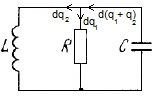
\includegraphics[height=30mm]{3_140.jpg}\\
	
	$g(t)={g}_{1}(t) + {g}_{2}(t)$\\
	$d({g}_{1}+{g}_{2})=d{g}_{1} + d{g}_{2}$\\
	По второму правилу Киргофа:\\
	$\frac{{Q}_{1}}{dt}R + \frac{{q}_{1}+{q}_{2}}{C}=0$\\
	$\frac{d^2q}{dt^2}+\frac{d({q}_{1}+{q}_{2})}{Cdt}$\\
	$\frac{{q}_{1}+{q}_{2}}{C}={\epsilon}_{C}=-\frac{d^2{q}_{2}}{dt}$\\
	$\frac{d^2({\varphi}_{1}+{\varphi}_{2})}{dt^2}+\frac{d({\varphi}_{1}+{\varphi}_{2})}{RCdt}+\frac{{q}_{1}+{q}_{2}}{LC}=0$\\
	${\omega}_{0}^2=\frac{1}{LC}; \beta = \frac{1}{2RC}$\\
	$\omega=\sqrt{\frac{1}{LC} - \frac{1}{4R^2C^2}}$\\
}

